\subsection{Entity System}
\label{entitysystem}
Die FM3D-Engine verwendet ein \textit{Entity-Component-System} um Objekte eines Spieles zu verwalten. Im Gegensatz zu einem vererbungs-basierten Entity-System ist dieses sehr flexibel. 
Die Grundidee besteht darin, die \textit{Daten} und \textit{Logik} eines Entities aufzuteilen. Hierfür werden alle Daten eines Entities (alle Attribute eines Entities) in Komponenten geschrieben. %removed by max Variablen -> Attribute
Die Logik (Methoden, die das Entity ausführen soll) wird in einen Manager geschrieben. 
Ein Entity kann beliebig viele verschiedene Komponenten besitzen und sie können während der Laufzeit beliebig hinzugefügt oder entfernt werden. Jedoch kann ein Entity immer nur einen Komponente eines Typs enthalten. 
Der Manager führt dann bei jedem Update oder bei bestimmten Events eine Methode, das die vom Manager benötigten Komponenten enthält, für jedes Entity aus.

Alle Entities werden in einer \textit{Entity-Collection} gespeichert. Diese ist eine Sammlung von Entities, welche dafür zuständig ist neue Entities zu erstellen und alte zu löschen. Wenn ein Entity zerstört wird, so wird dieses nicht aus dem Speicher gelöscht. Es bleibt weiterhin in der Entity-Collection gespeichert. 
Wenn dann ein neues Entity erstellt wird, so muss nicht neuer Speicher angefragt werden und das bereits vorhandene aber "'gelöschte"` Entity kann nun wieder verwendet werden. Dies ermöglicht es sehr viel zeitsparender und effizienter eine hohe Anzahl von Entities zu erstellen und wieder zu löschen. 
Mit Komponenten verhält es sich genauso. In der \textit{Entity-Collection} werden alle zerstörten Komponenten gespeichert. Diese werden solange gespeichert, bis eine neue Komponente des gleichen Typs erstellt wird. Das gesamte Entity-System befindet sich im Namespace \textit{EntitySystem} um es vom restlichen Code abzutrennen.

Bevor wir auf die wichtigsten Klassen des Entity-Systems eingehen, müssen erst einige Hilfsklassen erläutert werden.
\todo[inline]{Erklärung von Events}

Dies wird im Code durch die folgende Klassenstruktur ermöglicht. Die Hauptklasse Entity besitzt einen Container mit Komponenten, welche nach ihrer ID sortiert sind. Um auf eine Komponente zuzugreifen, benötigt man nur die ID dieser in Form eines 32-Bit Integer. Auf diese kann man mit der Hilfsklasse \textit{ComponentIds} zugreifen. 
Diese Klasse enthält eine statische Variable, die jedes Mal bei einer neuen ID erhöht wird. Auf die ID kann dann mit der statischen Template-Methode Get() zugegriffen werden.
 
Um ein Entity zu erstellen benötigt man ein Objekt der Klasse \textit{EntityCollection}. Mit der Entity-Klasse selbst kann kein ein Objekt erstellt werden.  
Die \textit{EntityCollection} enthält eine \textit{Map} mit bereits gelöschten Komponenten um diese wiederverwenden zu können. 
Alle Komponenten müssen nach ihrer ID sortiert werden, da nur Komponenten, die mit dem neuen Typ übereinstimmen und daher die gleiche Speichergröße und Variablen haben, für den neuen Komponenten verwendet werden können.

\begin{figure}
	\begin{center}
		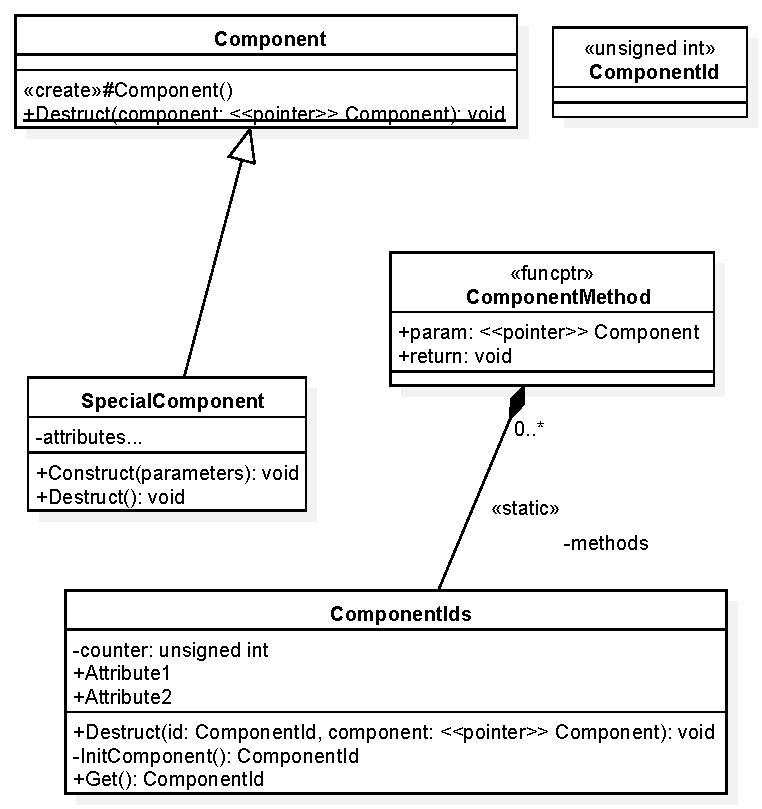
\includegraphics[width=\textwidth]{03unserprogramm/Engine/SpecialComponent.pdf}
		Die Klasse SpecialComponent ist eine Beispiel-Klasse für einen benutzererstellten Komponenten. Hierbei ist attributes für tatsächliche Variablen auszutauschen und parameters für die Parameter, die der Komponent benötigt um initialisiert zu werden. Es können gegebenenfalls auch mehrere Überladungen der Construct-Methode erstellt werden.
		\caption{Klassendiagramm der Component-Klassen}\label{ClassDiagramComponents}
	\end{center}
\end{figure}

Möchte man eine neue Komponente erstellen, so muss man eine Klasse erstellen, die von der Klasse Component erbt. Die Component-Klasse ist eine leere Klasse und dient nur dazu, verschiedene Komponenten auf eine allgemeine Weise zu speichern. 
\todo[inline]{KOMISCHER SATZ: START}
Wenn eine neue Komponente erstellt wird nicht unbedingt der Konstruktor aufgerufen wird, wenn ein alter Komponent wieder verwendet werden kann, muss jede Klasse, die von Component erbt die Methode Construct mit beliebigen Parametern enthalten, sowie die Methode Destruct ohne Parameter. 
\todo[inline]{KOMISCHER SATZ: ENDE}
Da Vererbung in diesem Fall einen großen Geschwindigkeitsverlust bewirken würde, muss die \textit{Construct}-Methode mit Hilfe von Templates aufgerufen werden. Bei der \textit{Destruct}-Methode ist dies leider nicht so einfach möglich, da der Datentyp zum Zeitpunkt der Zerstörung nicht mehr bekannt ist muss ein Funktions-Pointer für jeden Komponenten-Typ gespeichert werden. Dieser zeigt auf eine Funktion, welche einen \textit{Component}-Pointer erst zu dem spezifischen Komponenten-Pointer casted und dann die Destruct-Methode aufruft. Diese Funktion ist eine statische Template-Methode in der Component-Klasse. Mit dem Template-Parameter ist es möglich diese Methode für verschiedene Komponenten zu verwenden. Der Pointer wird in einem Objekt der Klasse \textit{EntityIds} gespeichert und kann verwendet werden, indem die statische Methode \textit{Destruct} aufgerufen wird, der sowohl die Komponente, als auch die ID übergeben wird. 
Er wird beim erstmaligen aufrufen der Methode Get() für jeden Komponent-Typ mit der Methode InitComponent() erstellt. Diese Klassen sind in \cref{ClassDiagramComponents} dargestellt.

Ein Manager ist eine Klasse, die von der Basisklasse \textit{Manager} erbt. 
\todo[inline]{Erklärung des Managers}